\section{Relations Groupes/Sessions}

Afin de clarifier les concepts de groupes de processus et de sessions, l'exemple de code shell ci-dessous offre une opportunité pratique pour illustrer leur interaction.


\begin{lstlisting}
$ echo $$ # PID du shell
1121
$ yes "data" | head -n 1000000000 > /dev/null &  # 2 process en background
[1] 1023
$ ps -o 'pid,ppid,pgid,sid,cmd' # 1 process en foreground
  PID    PPID    PGID     SID CMD
 1121    1117    1121    1121 bash
 1146    1121    1146    1121 yes data
 1147    1121    1146    1121 head -n 1000000000
 1148    1121    1148    1121 ps -o 'pid,ppid,pgid,sid,cmd'
\end{lstlisting}

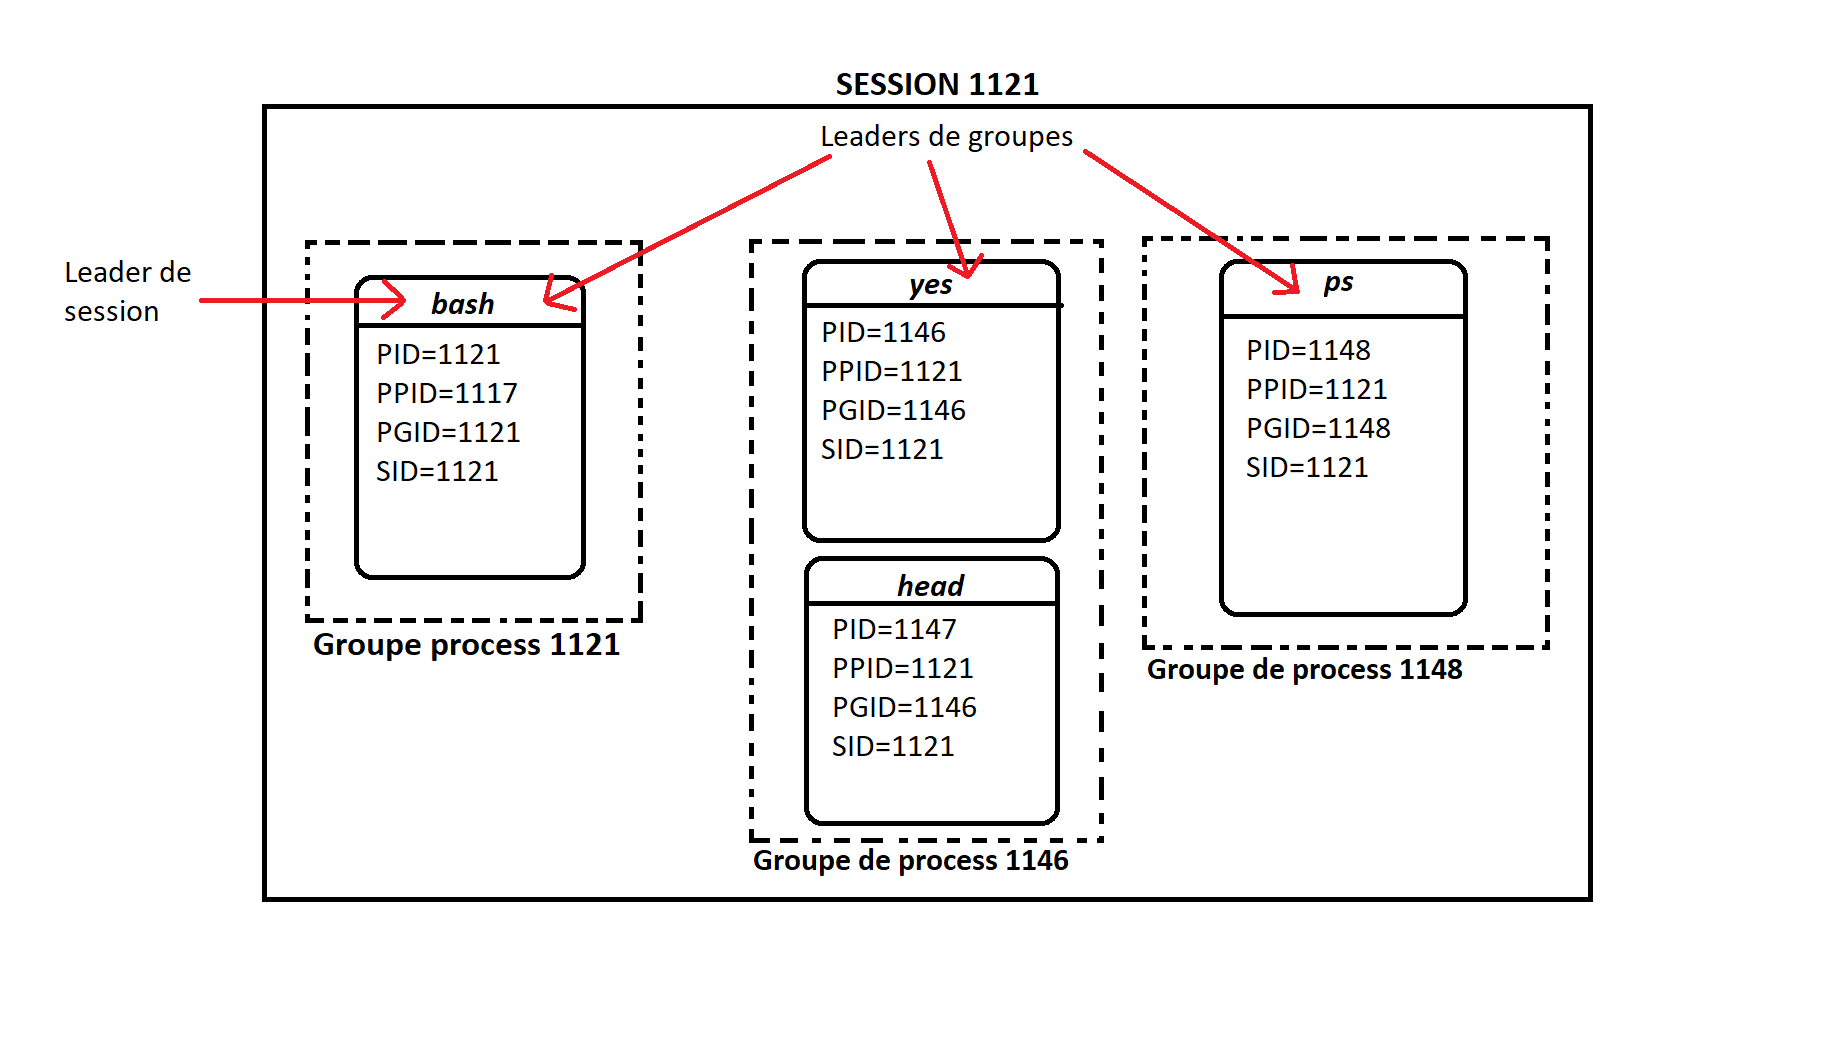
\includegraphics[width=1\textwidth]{img/relationshipSchema.png}